\paragraph*{Objective} \hfill \\

\paragraph*{Results and procedure} \hfill\\
Following values are given by:
\begin{align*}
R&= 1k\Omega	&	D&= 1N4001	&	E&=2v\,\,(i_{max}=350mA)	
\end{align*}

Measurements of the diode and resistor voltage and current for different resistors can be seen in the table below:
\begin{table}[H]
	\centering
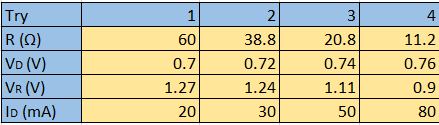
\includegraphics[width=0.7\textwidth]{./images/Kacper/31.png}
	\caption{Measurements for diode and resistor}
\end{table}
I-V characteristics of the diode can be seen below:
\begin{figure}[H]
	\centering
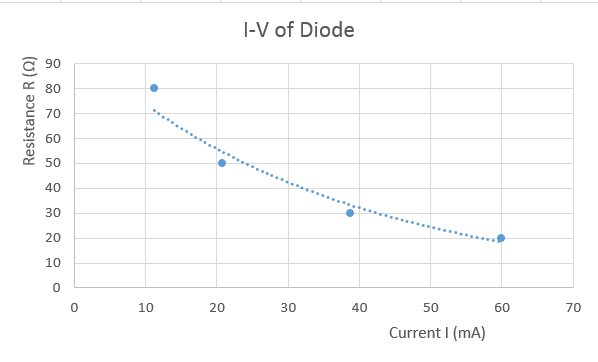
\includegraphics[width=1\textwidth]{./images/Kacper/31a.png}
	\caption{I-V characteristics for the diode}
\end{figure} 

\begin{flushleft}
I-V characteristics of the resistor can be seen below:
\end{flushleft}
\begin{figure}[H]
	\centering
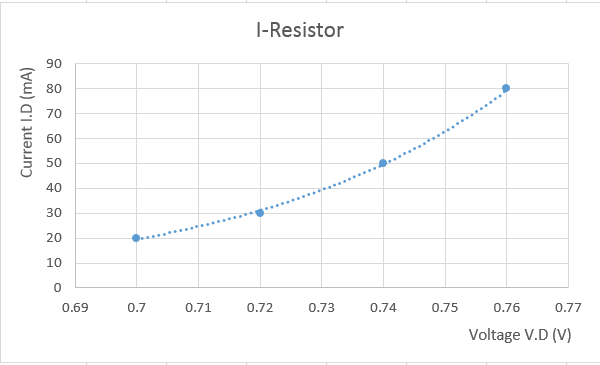
\includegraphics[width=1\textwidth]{./images/Kacper/31b.png}
	\caption{I-V characteristics for the resistor}
\end{figure}

\paragraph*{Conclusion} \hfill \\